\chapter{Introdução}\label{ch:intro}

As aplicações dos Veículos Aéreos Não Tripulados (\sigla{VANT}{Veículos Aéreos Não Tripulados}s) há décadas atraem pesquisadores de diversas partes do mundo e tem gerado muitas pesquisas. Na última década, os avanços em materiais, componentes eletrônicos, sensores e baterias permitiram grandes avanços no desenvolvimento destes veículos. A utilização de VANTs permite retirar o ser humano de condições de alta periculosidade e permitir um maior grau de liberdade e flexibilidade, abrindo possibilidades em tarefas que seriam impraticáveis para um veículo tripulado.

Entre os diversos tipos de VANTs, os helicópteros tem grande destaque, em especial os elétricos. Classificados como \sigla{VTOL}{Vertical Take-Off and Landing} (do inglês, \textit{Vertical Take-Off and Landing}), eles se diferenciam pelas seguintes características: 1) possui alta capacidade de carga; 2) possui seis graus de liberdade\footnote{O helicóptero possui seis graus de liberdade: rotação e translação nos eixos X, Y e Z.}, que permite maior manobrabilidade; 3) capacidade de miniaturização; 4) precisam de pouco espaço para pouso e decolagem; e 5) podem ser utilizados em ambientes internos e externos. No entanto, apresentam menor autonomia de voo em relação a outros VANTs e são mais difíceis de controlar.

Além dos helicópteros convencionais, com um rotor principal e um auxiliar na cauda, existem os multi-rotores, com dois ou mais rotores principais. A topologia com quatro rotores, dispostos em forma de ``+'' ou de ``X'' em uma plataforma, chamada de quadricóptero, é uma das mais pesquisadas devido à sua simplicidade mecânica e à desafiadora tarefa de estabilização de voo.

O primeiro quadricóptero foi construído pelos irmãos Louis e Jaques Breguet, em 1907, época em que se desenvolviam os primeiros aviões e helicópteros \cite{leishman00}. Devido a falta de estabilidade e de meios de controle, ele só foi capaz de levantar voo por alguns segundos. Nas décadas seguintes outras iniciativas conseguiram grandes avanços, superando os helicópteros convencionais em tempo de voo, contudo, apresentando complexos meios de controle. Nos anos seguintes, avanços significativos ocorreram nos helicópteros e o quadricópteros foram rapidamente ultrapassados e esquecidos.

O interesse por quadricópteros só foi reaparecer em meados de 1993, agora como VANT, no projeto Hoverbot, da Universidade de Michigan \cite{borestein93}. Este, como outros projetos desenvolvidos na sequência, sofreu com dificuldades de estabilização e não foi bem sucedido. Em 2002, na Universidade da Pensilvânia, houve um dos primeiros casos de sucesso com o projeto de \citeonline{altug02}. Seguido de vários outros, como \cite{niceCU04}, \cite{starmac04} e \cite{bouabdallah07}, tratando da estabilização de voo. Esses avanços em grande parte foram possíveis devido aos avanços dos sensores \sigla{MEMS}{Micro-Electro-Mechanical Systems}.

Alguns projetos conseguiram ótimos resultados utilizando realimentação visual para estimar a posição do veículo, como é o caso das equipes do Laboratório GRASP, da Universidade da Pensilvânia, e da Flying Machine Arena, dos Institutos Federais de Tecnologia da Suíça. Suas capacidades incluem manobras em alta velocidade, apresentações musicais e captura de bolas em voo. No entanto, estes veículos não são autônomos e requerem um processamento externo \cite{Lupashin2010, michael2010}.

No Brasil poucos trabalhos foram publicados nesse tema. A dissertação de mestrado de \citeonline{melo2010}, da Universidade Federal do Espírito Santo, propõe um quadricóptero como plataforma para desenvolvimento de algoritmos de controle e em \citeonline{lopes2011}, o modelo matemático de um quadricóptero é utilizado para simular e avaliar técnicas de controle.

Na UTFPR, uma tentativa de construção de um quadricóptero foi realizada na disciplina Oficinas de Integração 2, do curso de Engenharia de Computação, por \citeonline{oficinas2}. Apesar de não bem sucedida, a iniciativa despertou o interesse local, a exemplo do prof. Hugo Vieira, que comprou os materiais necessários para construção em um projeto futuro. Esses materiais, gentilmente cedidos, agora serão utilizados na elaboração deste projeto.

Além das aplicações militares, de vigilância e busca e resgate, que incentivaram as pesquisas inicias nessa área, há uma grande ramo de aplicações dos quadricópteros para fins acadêmicos. Estes podem ser utilizados ensino de diversas áreas, como: algoritmos de controle, para estabilização; inteligência artificial, para detecção e desvio de obstáculos; processamento de imagens; sistemas multi-agentes, no estudo de comportamento coletivo; entre outras. Este projeto seria o primeiro passo para posterior utilização em outros projetos.


\section{Objetivos geral e específicos}

Esse trabalho tem como objetivo desenvolver um quadricóptero elétrico autônomo, capaz de voar a uma altura fixa e evitar colisões. Esse objetivo principal pode ser dividido nos seguintes objetivos específicos:

\begin{itemize}
\item projetar e montar a estrutura física;
\item modelar o sistema;
\item projetar e implementar o sistema de comunicação;
\item projetar e construir o sistema embarcado;
\item projetar e implementar o sistema de controle;
\item idealizar e conduzir experimentos reais de teste de navegação.
\end{itemize}


\section{Organização do documento}

Esse documento será organizado da seguinte forma. O Capítulo \ref{cap:funda} apresentará inicialmente uma breve história do desenvolvimento dos quadricópteros. Em seguida, são apresentados os trabalhos correlatos recentes, com o intuito de situar este trabalho no estágio atual do conhecimento. A metodologia utilizada se encontra no Capítulo \ref{cap:metod}, nele são descritas todas as etapas para o desenvolvimento do projeto. No Capítulo \ref{cap:recur} são listados os recursos de \textit{software} e \textit{hardware} utilizados, bem como a forma de aquisição de cada um. O estudo de viabilidade e um cronograma preliminar são apresentados no Capítulo \ref{cap:viabi} e, por fim, no Capítulo \ref{cap:concl} encontra-se a conclusão da proposta do trabalho de conclusão de curso.

\section{Exemplos gerais que podem ser usados no TCC}\label{subsec:ExemplosLatex}



\subsubsection{Titulo C}\label{ssubsec:tituloc}

.....Teste de citaç\~ao de autor: ~\cite{AikesJunior2011}. Podendo ser também \citeonline{AikesJunior2011}, dependendo do contexto.
.....Teste de referência de seç\~ao, cap\'itulo ou figura: Capítulo~\ref{ch:intro} = (Introduç\~ao), Figura~\ref{fig:tux_laplace} (Figura Tux), Tabela~\ref{tab:tab_exemplo} (Tabela).

Exemplo de Equação não numerada: $3 \times \sum_{i=0}^{j}\Delta$.

A Equação~\ref{eq:segundoGrau} é um exemplo de uma equação numerada:
\begin{equation}
x = \dfrac{-b \pm \sqrt{ \Delta}}{2 \times a}
\label{eq:segundoGrau}
\end{equation}


$3 \times 3$
$\boldmath{ 3 \times 3}$

Modelo de chamada de figura.

\begin{figure}[htb]
	\centering
	
\includegraphics[width=0.4\textwidth]{Imagens/tux_laplace.png} % <- formatos PNG, JPG e PDF
	\caption[Texto que vai aparecer na lista de fig.]{Texto que vai aparecer embaixo da imagem.}
\fonte{\cite{oge1999}}%citaç\~ao do livro onde pegou a figura	
	\label{fig:tux_laplace}
\end{figure}

Modelo de chamada de subfigures:
\begin{figure}[!htb]
\centering
\subfigure[]{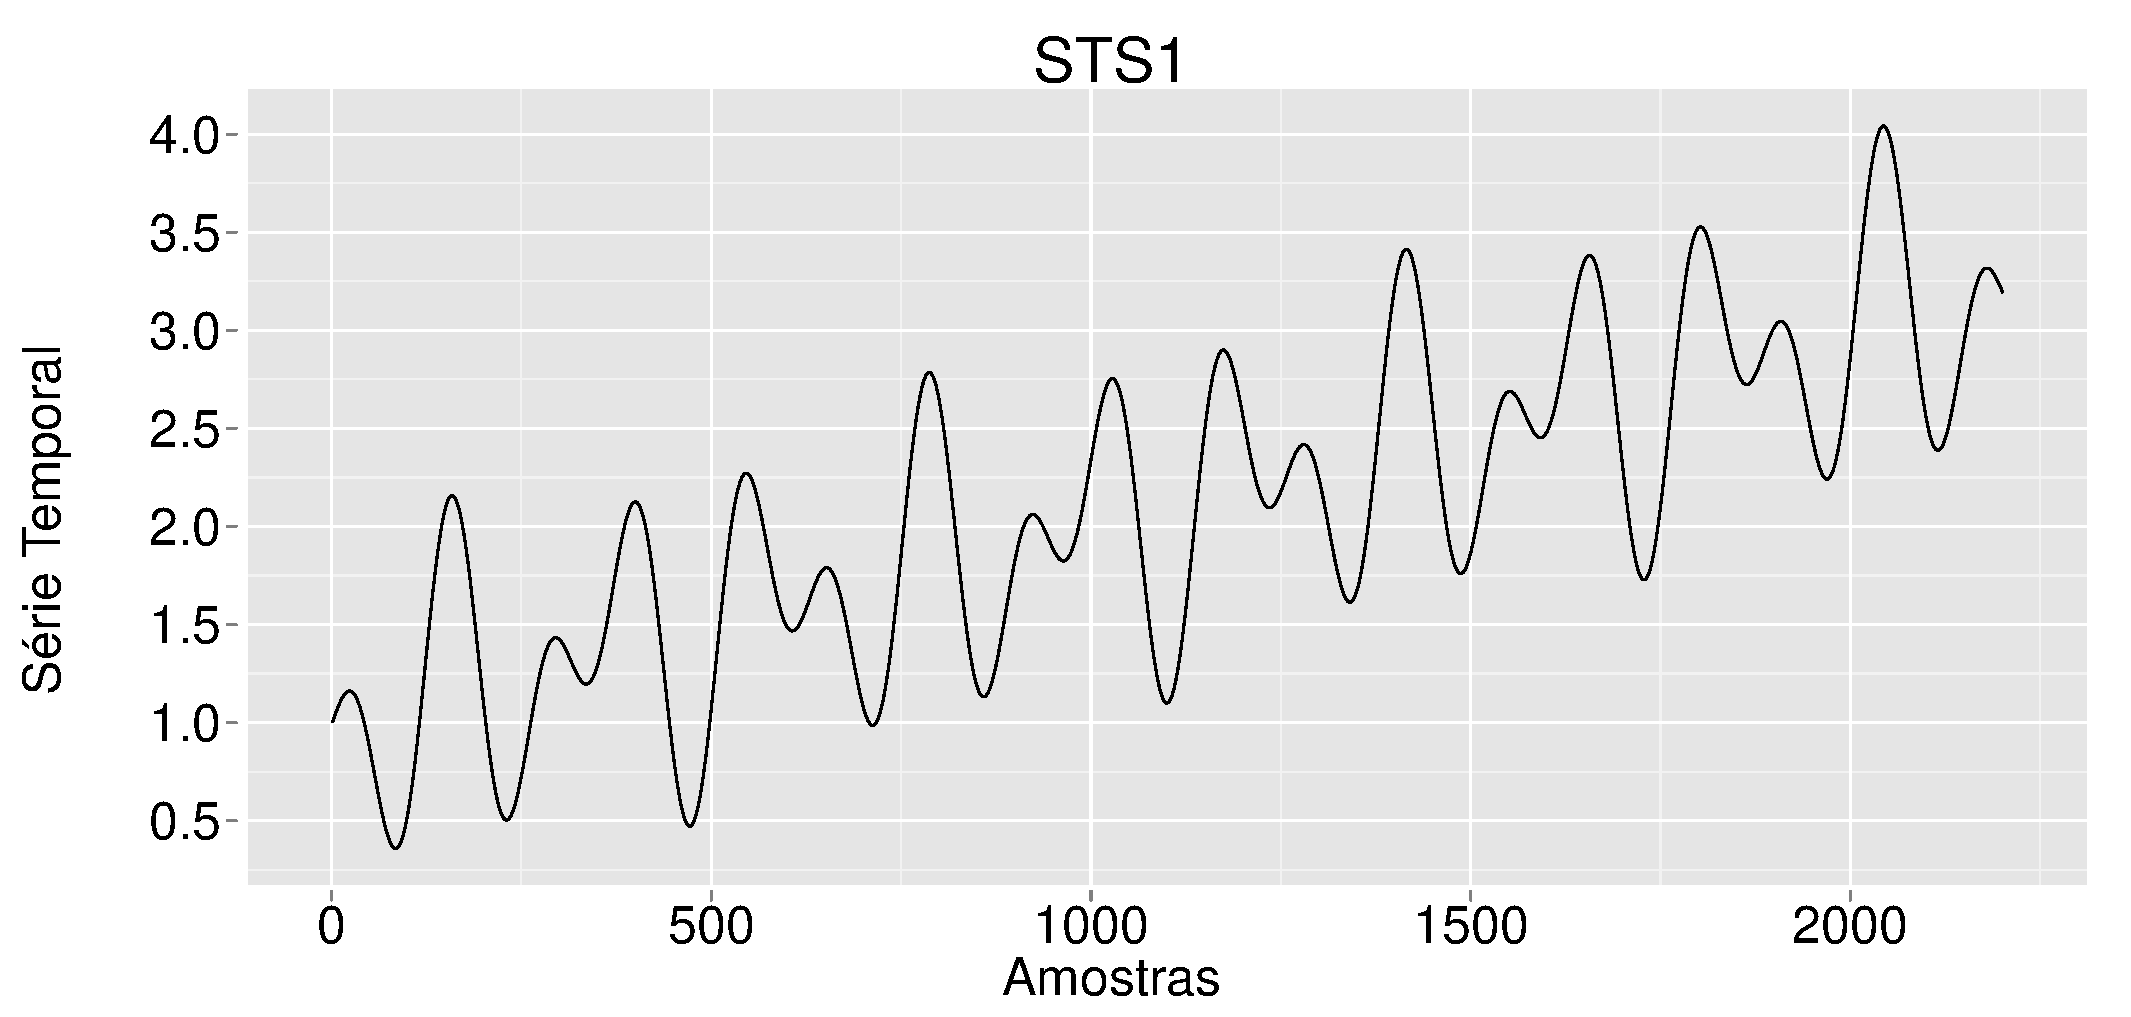
\includegraphics[width=0.49\textwidth]{Imagens/Arta1.pdf}}
\subfigure[]{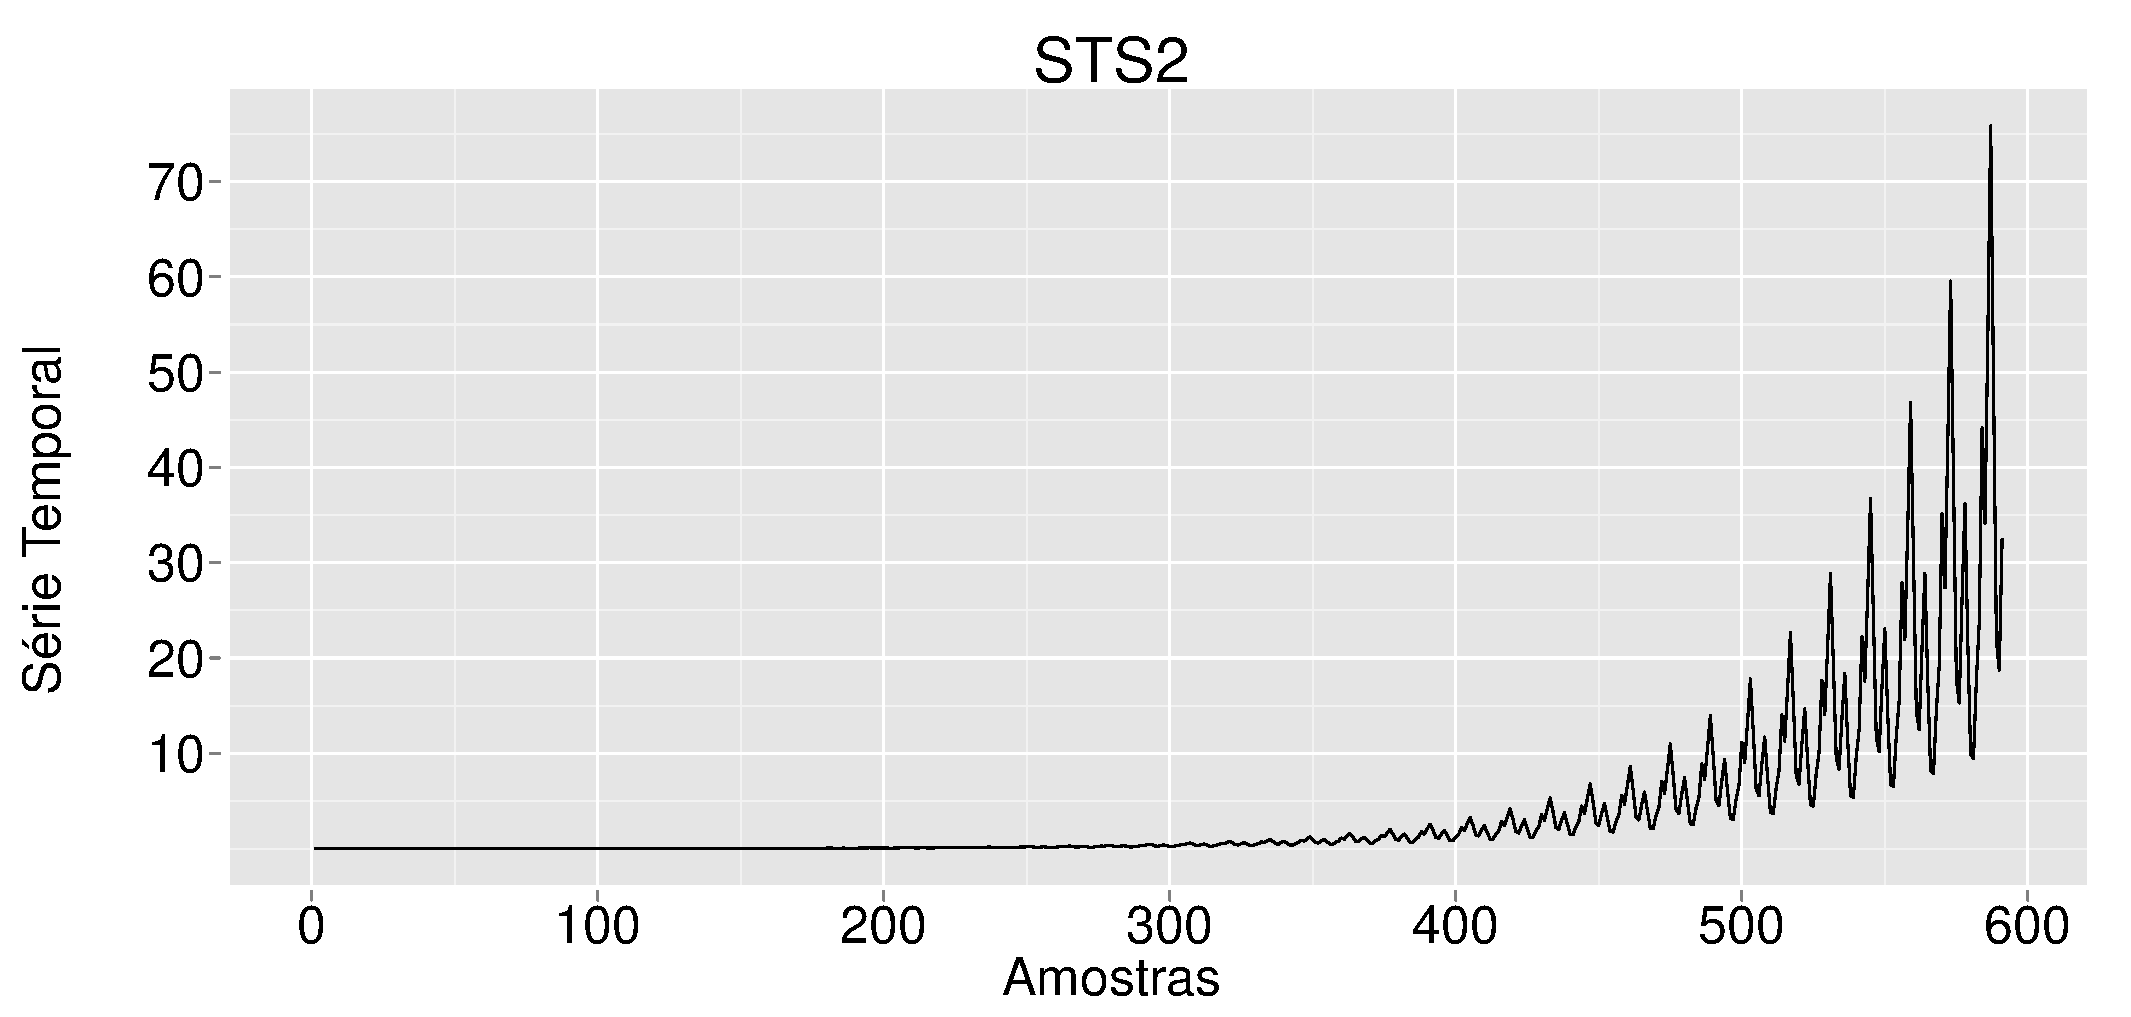
\includegraphics[width=0.49\textwidth]{Imagens/Arta2.pdf}}
\subfigure[]{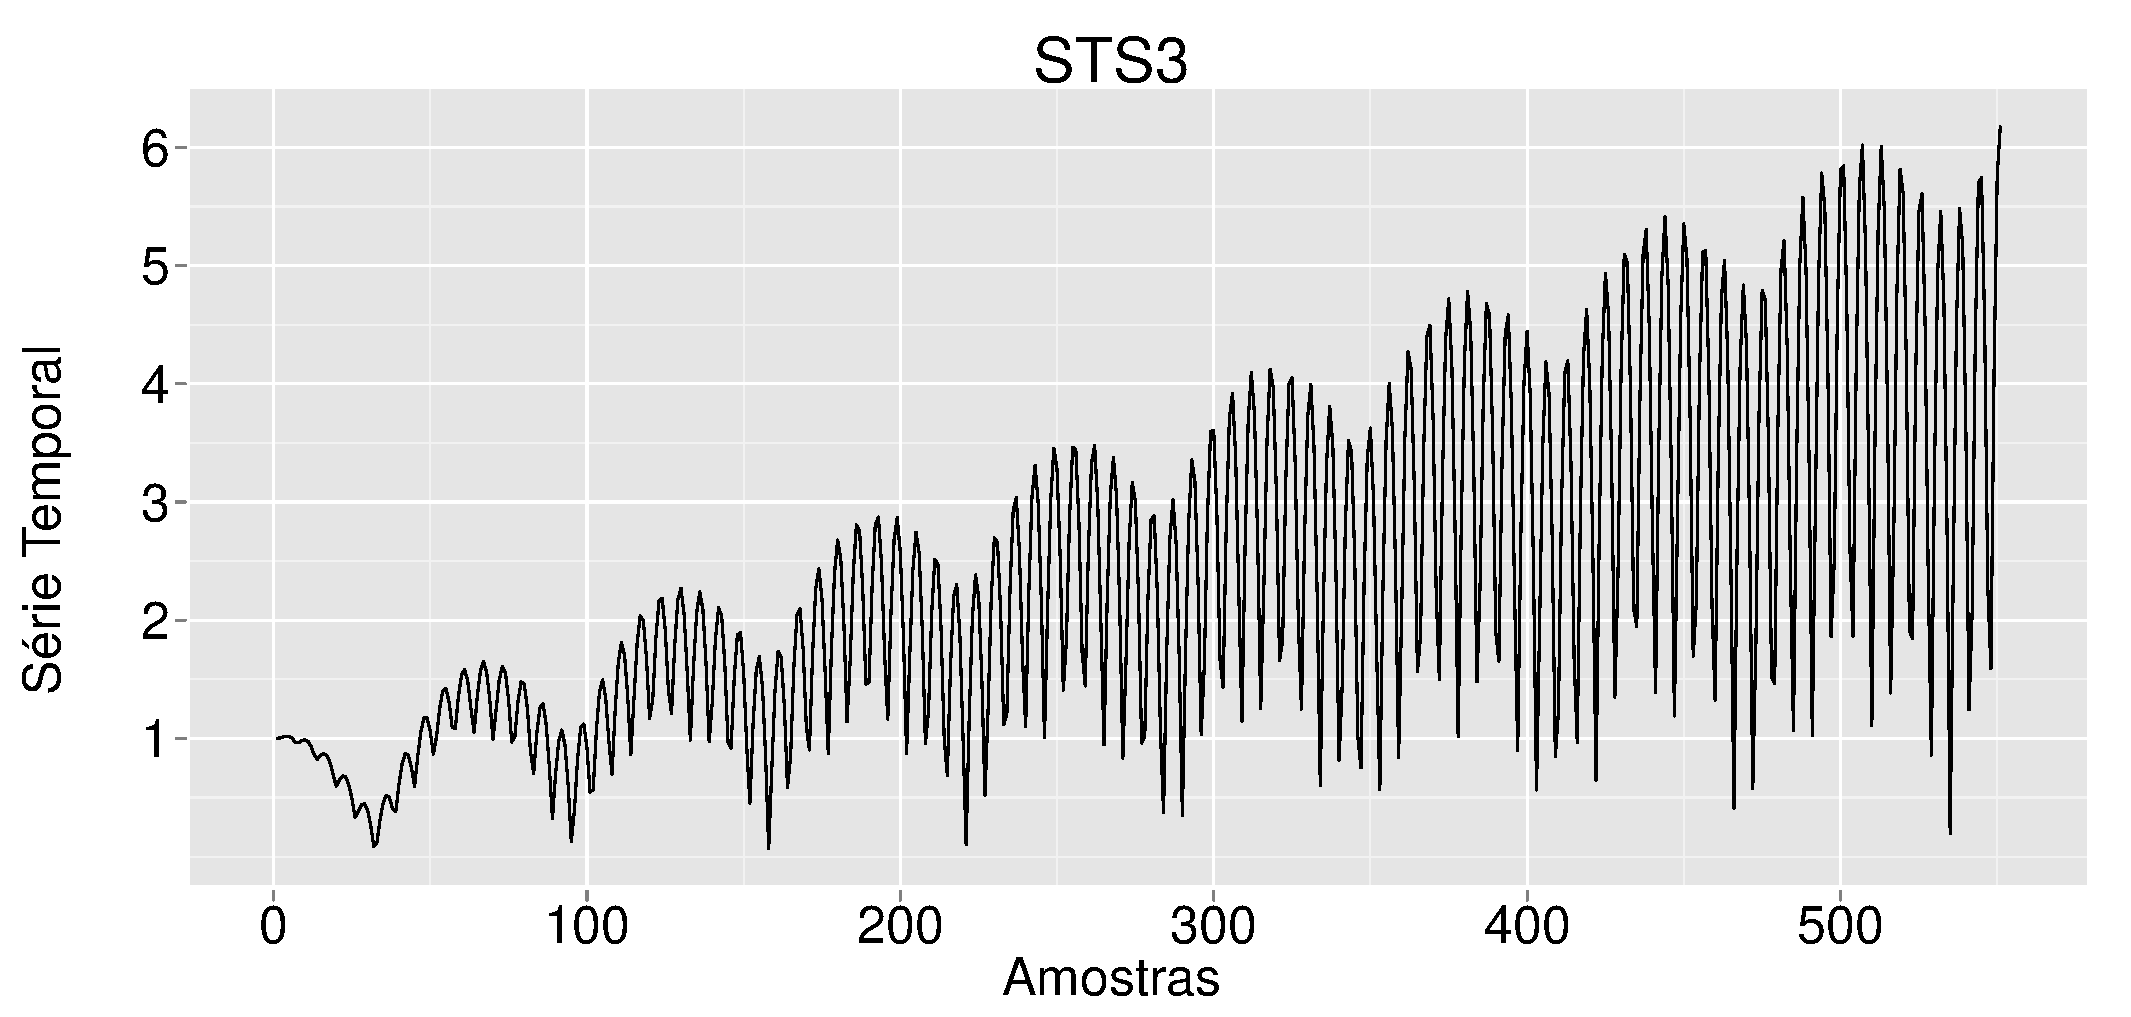
\includegraphics[width=0.49\textwidth]{Imagens/Arta3.pdf}}
\caption[Séries temporais artificiais geradas através de modelos sazonais]{Séries temporais artificiais geradas através de modelos sazonais: (a) STS1, (b) STS2 e (c) STS3.}
\label{fig:SeriesA}
\end{figure}


Modelo de tabela.
\begin{table}[!htb]
	\centering	
	\label{tab:tab_exemplo}
\begin{tabular}{|c|c|c|}
\hline 
Coluna 1 & Coluna 2 & Coluna 3 \\ 
\hline 
Conteúdo 1 & Conteúdo 2 & Conteúdo 3 \\ 
\hline 
\end{tabular} 
\caption[Texto da lista de tabelas]{Texto abaixo da tabela.}
\end{table}

Exemplo de algoritmo:
No Algoritmo~\ref{alg:kNNTSP}~\cite{Ferrero2009} é apresentado o pseudocódigo, em alto nível, do algoritmo, onde:
\begin{itemize}
\item $Z$ representa a ST utilizada;
\item $w$ representa o tamanho da janela para busca das sequências;
\item $M_s$ representa a medida de similaridade utilizada;
\item $C_k$ representa o critério utilizado para a seleção dos vizinhos próximos;
\item $k$ representa a quantidade de vizinhos mais próximos; e
\item $f$ representa a função de previsão utilizada para o cálculo do valor futuro.
\end{itemize}

\begin{algorithm}[hbtp]
\caption{\textit{$k$-NNTSP}.}
\label{alg:kNNTSP}
\Entrada{$Z$, $w$, $M_s$, $C_k$, $k$, $f$}
\Saida{$\hat{z}_{n+1};$}
\Inicio{
// Construção do conjunto de séries de treinamento $S$ a partir da série temporal $Z$ 

// e tamanho de janela $w$

$S \leftarrow series\_de\_treinamento(Z, w);$

// Definição da sequência de referência $U$

$U \leftarrow (z_n);$

// Obtenção das $k$ sequências mais próximas a $U$ contidas em $S$, considerando a

// medida de similaridade $M_s$ e o critério de seleção de vizinhos próximos $C_k$

$S' \leftarrow vizinhos\_proximos(S, U, M_s, C_k, k);$

// Cálculo do valor futuro da sequências de referências, utilizando $f(S')$

$\hat{z}_{n+1} \leftarrow f(S');$

\Retorna{$\hat{z}_{n+1}$}
}
\end{algorithm}

Exemplo de trecho de código.
\begin{lstlisting}[caption=Teste de Hello World]
/**
* comentario
*/
public class HelloWorldApp {
  public static void main (String argv[])
  {
    // Comentario
    System.out.println("Hello World!");
  }
}
\end{lstlisting}

Exemplo de tabela que ocupa mais de uma página (long tables):

\tablecaption{Características das ST disponíveis pela \textit{NNGC I}.} 
\tablefirsthead{\hline
    \hline
    \multicolumn{1}{c|}{{\scriptsize \textbf{Id}}} & \multicolumn{1}{c|}{{\scriptsize \textbf{Base de Dados}}} & \multicolumn{1}{c|}{{\scriptsize \textbf{Aquisição}}} & \multicolumn{1}{c|}{\scriptsize {\textbf{Tamanho}}} & \multicolumn{1}{c|}{{\scriptsize \textbf{Início }}} & \multicolumn{1}{c}{{\scriptsize \textbf{Término}}} \\
    \hline}
\tablehead{\multicolumn{6}{c}
    {{\tablename\ \thetable{ -- Características das ST disponíveis pela \textit{NNGC I}.}}} \\
    \hline 
    \hline
    \multicolumn{6}{r}
    {\scriptsize Continuação da página anterior.}\\
    \hline
    \multicolumn{1}{c|}{{\scriptsize \textbf{Id}}} & \multicolumn{1}{c|}{{\scriptsize \textbf{Base de Dados}}} & \multicolumn{1}{c|}{{\scriptsize \textbf{Aquisição}}} & \multicolumn{1}{c|}{\scriptsize {\textbf{Tamanho}}} & \multicolumn{1}{c|}{{\scriptsize \textbf{Início }}} & \multicolumn{1}{c}{{\scriptsize \textbf{Término}}}\\}
\tabletail{\hline 
\multicolumn{6}{r}
           {\scriptsize Continua na página seguinte.}\\
            }
\tablelasttail{\hline \hline}
%\xentrystretch{-0.15}
\begin{center}
\begin{xtabular}{c|c|c|c|c|c}
    {\scriptsize 1.B-001} & {\scriptsize 1.B}   & {\scriptsize Quaternal} & {\scriptsize 40}   & {\scriptsize jan-1993} & {\scriptsize abr-2002} \\ \hline
    {\scriptsize 1.B-002} & {\scriptsize 1.B}   & {\scriptsize Quaternal} & {\scriptsize 31}   & {\scriptsize jan-1990} & {\scriptsize mar-1997} \\ \hline
    {\scriptsize 1.B-003} & {\scriptsize 1.B}   & {\scriptsize Quaternal} & {\scriptsize 148}   & {\scriptsize jan-1967} & {\scriptsize abr-2003}\\ \hline
    {\scriptsize 1.B-004} & {\scriptsize 1.B}   & {\scriptsize Quaternal} & {\scriptsize 148}   & {\scriptsize jan-1967} & {\scriptsize abr-2003} \\ \hline
    {\scriptsize 1.B-005} & {\scriptsize 1.B}   & {\scriptsize Quaternal} & {\scriptsize 148}   & {\scriptsize jan-1967} & {\scriptsize abr-2003} \\ \hline
    {\scriptsize 1.B-006} & {\scriptsize 1.B}   & {\scriptsize Quaternal} & {\scriptsize 108}   & {\scriptsize jan-1977} & {\scriptsize abr-2003} \\ \hline
    {\scriptsize 1.B-007} & {\scriptsize 1.B}   & {\scriptsize Quaternal} & {\scriptsize 108}   & {\scriptsize jan-1977} & {\scriptsize abr-2003} \\ \hline
    {\scriptsize 1.B-008} & {\scriptsize 1.B}   & {\scriptsize Quaternal} & {\scriptsize 148}   & {\scriptsize jan-1967} & {\scriptsize abr-2003} \\ \hline
    {\scriptsize 1.B-009} & {\scriptsize 1.B}   & {\scriptsize Quaternal} & {\scriptsize 148}   & {\scriptsize jan-1967} & {\scriptsize abr-2003} \\ \hline
    {\scriptsize 1.B-010} & {\scriptsize 1.B}   & {\scriptsize Quaternal} & {\scriptsize 148}   & {\scriptsize jan-1967} & {\scriptsize abr-2003} \\ \hline
    {\scriptsize 1.B-011} & {\scriptsize 1.B}   & {\scriptsize Quaternal} & {\scriptsize 148}   & {\scriptsize jan-1967} & {\scriptsize abr-2003} \\ \hline
    {\scriptsize 1.C-001} & {\scriptsize 1.C}   & {\scriptsize Mensal} & {\scriptsize 48 }   & {\scriptsize jan-1999} & {\scriptsize dez-2002} \\ \hline
    {\scriptsize 1.C-002} & {\scriptsize 1.C}   & {\scriptsize Mensal} & {\scriptsize 48 }   & {\scriptsize jan-1999} & {\scriptsize dez-2002} \\ \hline
    {\scriptsize 1.C-003} & {\scriptsize 1.C}   & {\scriptsize Mensal} & {\scriptsize 198}   & {\scriptsize set-1987} & {\scriptsize fev-2004} \\ \hline
    {\scriptsize 1.C-004} & {\scriptsize 1.C}   & {\scriptsize Mensal} & {\scriptsize 172}   & {\scriptsize jan-1990} & {\scriptsize abr-2004} \\ \hline
    {\scriptsize 1.C-005} & {\scriptsize 1.C}   & {\scriptsize Mensal} & {\scriptsize 118}   & {\scriptsize out-1993} & {\scriptsize jul-2003} \\ \hline
    {\scriptsize 1.C-006} & {\scriptsize 1.C}   & {\scriptsize Mensal} & {\scriptsize 118}   & {\scriptsize out-1993} & {\scriptsize jul-2003} \\ \hline
    {\scriptsize 1.C-007} & {\scriptsize 1.C}   & {\scriptsize Mensal} & {\scriptsize 118}   & {\scriptsize out-1993} & {\scriptsize jul-2003} \\ \hline
    {\scriptsize 1.C-008} & {\scriptsize 1.C}   & {\scriptsize Mensal} & {\scriptsize 57 }   & {\scriptsize abr-1998} & {\scriptsize dez-2002} \\ \hline
    {\scriptsize 1.C-009} & {\scriptsize 1.C}   & {\scriptsize Mensal} & {\scriptsize 227}   & {\scriptsize jan-1983} & {\scriptsize nov-2001} \\ \hline
    {\scriptsize 1.C-010} & {\scriptsize 1.C}   & {\scriptsize Mensal} & {\scriptsize 132}   & {\scriptsize abr-1993} & {\scriptsize mar-2004} \\ \hline
    {\scriptsize 1.C-011} & {\scriptsize 1.C}   & {\scriptsize Mensal} & {\scriptsize 228}   & {\scriptsize mar-1986} & {\scriptsize fev-2005} \\ \hline
    {\scriptsize 1.D-001} & {\scriptsize 1.D}   & {\scriptsize Semanal} & {\scriptsize 527 }  & {\scriptsize 02-jan-1995} & {\scriptsize 31-jan-2005} \\ \hline
    {\scriptsize 1.D-003} & {\scriptsize 1.D}   & {\scriptsize Semanal} & {\scriptsize 437 }  & {\scriptsize 03-jan-1997} & {\scriptsize 13-mai-2005} \\ \hline
    {\scriptsize 1.D-004} & {\scriptsize 1.D}   & {\scriptsize Semanal} & {\scriptsize 549 }  & {\scriptsize 11-nov-1994} & {\scriptsize 13-mai-2005} \\ \hline
    {\scriptsize 1.D-005} & {\scriptsize 1.D}   & {\scriptsize Semanal} & {\scriptsize 437 }  & {\scriptsize 03-jan-1997} & {\scriptsize 13-mai-2005} \\ \hline
    {\scriptsize 1.D-006} & {\scriptsize 1.D}   & {\scriptsize Semanal} & {\scriptsize 618 }  & {\scriptsize 16-jul-1993} & {\scriptsize 13-mai-2005} \\ \hline
    {\scriptsize 1.D-007} & {\scriptsize 1.D}   & {\scriptsize Semanal} & {\scriptsize 618 }  & {\scriptsize 16-jul-1993} & {\scriptsize 13-mai-2005} \\ \hline
    {\scriptsize 1.D-008} & {\scriptsize 1.D}   & {\scriptsize Semanal} & {\scriptsize 548 }  & {\scriptsize 18-nov-1994} & {\scriptsize 13-mai-2005} \\ \hline
    {\scriptsize 1.D-009} & {\scriptsize 1.D}   & {\scriptsize Semanal} & {\scriptsize 548 }  & {\scriptsize 18-nov-1994} & {\scriptsize 13-mai-2005} \\ \hline
    {\scriptsize 1.D-010} & {\scriptsize 1.D}   & {\scriptsize Semanal} & {\scriptsize 593 }  & {\scriptsize 07-jan-1994} & {\scriptsize 13-mai-2005} \\ \hline
    {\scriptsize 1.D-011} & {\scriptsize 1.D}   & {\scriptsize Semanal} & {\scriptsize 594 }  & {\scriptsize 10-jan-1994} & {\scriptsize 23-mai-2005} \\ \hline
    {\scriptsize 1.E-001} & {\scriptsize 1.E}   & {\scriptsize Diária} & {\scriptsize 377}   & {\scriptsize 01-jan-2005} & {\scriptsize 12-jan-2006} \\ \hline
    {\scriptsize 1.E-002} & {\scriptsize 1.E}   & {\scriptsize Diária} & {\scriptsize 377}   & {\scriptsize 01-jan-2005} & {\scriptsize 12-jan-2006} \\ \hline
    {\scriptsize 1.E-004} & {\scriptsize 1.E}   & {\scriptsize Diária} & {\scriptsize 466}   & {\scriptsize 07-fev-2003} & {\scriptsize 17-mai-2004} \\ \hline
    {\scriptsize 1.E-005} & {\scriptsize 1.E}   & {\scriptsize Diária} & {\scriptsize 716}   & {\scriptsize 01-jan-2002} & {\scriptsize 17-dez-2003} \\ \hline
    {\scriptsize 1.E-006} & {\scriptsize 1.E}   & {\scriptsize Diária} & {\scriptsize 502}   & {\scriptsize 01-jan-2002} & {\scriptsize 17-mai-2003} \\ \hline
    {\scriptsize 1.E-007} & {\scriptsize 1.E}   & {\scriptsize Diária} & {\scriptsize 502}   & {\scriptsize 01-jan-2002} & {\scriptsize 17-mai-2003} \\ \hline
    {\scriptsize 1.E-008} & {\scriptsize 1.E}   & {\scriptsize Diária} & {\scriptsize 747}   & {\scriptsize 01-nov-2003} & {\scriptsize 16-nov-2005} \\ \hline
    {\scriptsize 1.E-009} & {\scriptsize 1.E}   & {\scriptsize Diária} & {\scriptsize 747}   & {\scriptsize 01-nov-2003} & {\scriptsize 16-nov-2005} \\ \hline
    {\scriptsize 1.E-010} & {\scriptsize 1.E}   & {\scriptsize Diária} & {\scriptsize 654}   & {\scriptsize 01-jul-2003} & {\scriptsize 14-abr-2005} \\ \hline
    {\scriptsize 1.E-011} & {\scriptsize 1.E}   & {\scriptsize Diária} & {\scriptsize 654}   & {\scriptsize 01-jul-2003} & {\scriptsize 14-abr-2005} \\ \hline
    {\scriptsize 1.F-003} & {\scriptsize 1.F}   & {\scriptsize Horária (5:00-24:00)} & {\scriptsize 1742}  & {\scriptsize 02-jan-2005} & {\scriptsize 29-mar-2005} \\ \hline
    {\scriptsize 1.F-004} & {\scriptsize 1.F}   & {\scriptsize Horária (5:00-24:00)} & {\scriptsize 902 }  & {\scriptsize 05-set-2005} & {\scriptsize 19-out-2005} \\ \hline
    {\scriptsize 1.F-005} & {\scriptsize 1.F}   & {\scriptsize Horária (5:00-24:00)} & {\scriptsize 902 }  & {\scriptsize 05-set-2005} & {\scriptsize 19-out-2005} \\ \hline
    {\scriptsize 1.F-006} & {\scriptsize 1.F}   & {\scriptsize Horária (5:00-24:00)} & {\scriptsize 1742}  & {\scriptsize 02-jan-2005} & {\scriptsize 29-mar-2005} \\ \hline
    {\scriptsize 1.F-007} & {\scriptsize 1.F}   & {\scriptsize Horária (5:00-24:00)} & {\scriptsize 1742}  & {\scriptsize 02-jan-2005} & {\scriptsize 29-mar-2005} \\ \hline
    {\scriptsize 1.F-008} & {\scriptsize 1.F}   & {\scriptsize Horária (5:00-24:00)} & {\scriptsize 1742}  & {\scriptsize 02-jan-2005} & {\scriptsize 29-mar-2005} \\ \hline
    {\scriptsize 1.F-009} & {\scriptsize 1.F}   & {\scriptsize Horária (5:00-24:00)} & {\scriptsize 902 }  & {\scriptsize 05-set-2005} & {\scriptsize 19-out-2005} \\ \hline
    {\scriptsize 1.F-010} & {\scriptsize 1.F}   & {\scriptsize Horária (5:00-24:00)} & {\scriptsize 902 }  & {\scriptsize 05-set-2005} & {\scriptsize 19-out-2005} \\ \hline
    {\scriptsize 1.F-011} & {\scriptsize 1.F}   & {\scriptsize Horária (5:00-24:00)} & {\scriptsize 902 }  & {\scriptsize 05-set-2005} & {\scriptsize 19-out-2005} \\ 
\end{xtabular}
\end{center}






